\documentclass[10pt]{scrartcl}
\usepackage[english]{babel}
\usepackage{multirow}
\usepackage[default]{opensans}
\usepackage{sfmath} % sans font also for math
\usepackage[binary-units = true]{siunitx}
\usepackage{graphicx}
% defining the paper layout that no text overlaps with the header
\usepackage[
  top=35mm,
  headheight=25mm,
  headsep=3mm,
  bottom=30mm,
  left=25mm,
  right=25mm
]{geometry}

\usepackage[verbose]{placeins}
\usepackage{subcaption}
\usepackage{latexsym}
\usepackage[centertags]{amsmath}
\usepackage{amssymb}
\usepackage[]{glossaries}

\graphicspath{{figures/}}
% custom header and footpage
\usepackage{scrpage2}
\pagestyle{scrheadings} % you have to set the custom layout
% Head
%\chead{}
%\ohead{\includegraphics[height=25mm]{figures/EUCALL.png}}
% Foot
%\ifoot{
\includegraphics[height=13.4mm]{figures/EU.png}} % left foot
\cfoot{%
  \begin{minipage}{100mm}%
    \begin{scriptsize}%
      \normalfont{This project has received funding from the}
      \textit{European Union’s Horizon 2020 research and innovation programme}
      \normalfont{under grant agreement No XXXXXX.}
    \end{scriptsize}%
  \end{minipage}%
} % center foot
\ofoot{\thepage} % right foot

\usepackage{booktabs}

%%%%%%%%%%%%%%%%%%%%%%%%%%%%%%%%%%%%%%%%%%%%%%%
%   BIBLIOGRAPHY SETTINGS
\usepackage[bibstyle=nature,sorting=none,maxnames=1000,eprint=false,
defernumbers=true, backend=biber]{biblatex}
\usepackage{chemformula}
\usepackage{hyperref}


%\renewcommand*\finalnamedelim{, and\addspace}
%\DeclareNameAlias{sortname}{last-first}
%\renewcommand{\newunitpunct}{, }

%\AtEveryBibitem{%
  %\clearfield{day}%
  %\clearfield{month}%
  %\clearfield{endday}%
  %\clearfield{endmonth}%
  %\clearfield{issn}%
  %\clearfield{issue}%
%}
%%convert titles to hyperlinks using doi
%\ExecuteBibliographyOptions{doi=true} \newbibmacro{string+doi}[1]{%
  %\iffieldundef{doi}{#1}{\href{http://dx.doi.org/\thefield{doi}}{#1}}}
  %\DeclareFieldFormat*{title}{\usebibmacro{string+doi}{\mkbibemph{#1}}}

%\addbibresource{urls.bib}
%\addbibresource{footnotes.bib}
%\addbibresource{library.bib}

%%%%%%%%%%%%%%%%%%%%%%%%%%%%%%%%%%%%%%%%%%%%%%%
% GLOSSARY SETTINGS
%\setacronymstyle{long-short}
%\input{glossary}
%\makeglossaries
%%%%%%%%%%%%%%%%%%%%%%%%%%%%%%%%%%%%%%%%%%%%%%%

% Zeilenabstand
\renewcommand{\baselinestretch}{1.2}


% sophisticated linking of references in the pdf and setting some options
\usepackage{url}                                                  % for correct typesettings of URLs
\usepackage{hyperref}                                             % for sophisticated linking of urls, dois, pictures, tables, etc.
\hypersetup{
    unicode=true,                                                 % non-Latin characters in Acrobat’s bookmarks
    pdftoolbar=true,                                              % show Acrobat’s toolbar?
    pdfmenubar=true,                                              % show Acrobat’s menu?
    pdffitwindow=false,                                           % window fit to page when opened
    pdfstartview={FitH},                                          % fits the width of the page to the window
    pdfauthor={C. Fortmann-Grote},                                           % author
    pdftitle={D5.3: Repository of documented jupyter notebooks and Oasys canvase },   % title
    pdfsubject={PaNOSC WP5 (ViNYL) Deliverable D5.3},                             % subject of the document
    pdfcreator={pdflatex},                                         % creator of the document
    pdfkeywords={PaNOSC, ViNYL, simulations, jupyter, simex, oasys, McStas,
    service},                                         % list of keywords
    pdfnewwindow=true,                                            % links in new PDF window
    colorlinks=true,                                              % false: boxed links; true: colored links
    linkcolor=blue,                                                % color of internal links (change box color with linkbordercolor)
    citecolor=blue,                                                % color of links to bibliography
    filecolor=blue,                                               % color of file links
    urlcolor=blue                                                 % color of external links
}

\begin{document}
\makeatletter
\begin{titlepage}
\thispagestyle{scrheadings}
\ohead{}
\ihead{}
\chead{}
\ifoot{}
\ofoot{}
\noindent%

\includegraphics[width=0.4\textwidth]{figures/PaNOSClogo_web_RGB_512x512.jpg}\\
\Huge{%
\renewcommand{\baselinestretch}{2.0}%
  \textbf{%
    Deliverable D5.3: Repository of documented jupyter notebooks and Oasys canvases\\
  }%
}%
\\
{%
\Large{%
  Mads Bertelsen,
  Stella d'Ambrumenil,
  Juncheng E,
  Aljo\v{s}a Hafner,
  Gergely Norbert Nagy,
  Shervin Nourbakhsh,
  Mousumi Upadhyay Kahaly,
  Carsten Fortmann-Grote
  \bigskip\\
  \bigskip\\
  \textbf{\today}%
}}%
\end{titlepage}
\makeatother

%\tableofcontents
\section{Simulation infrastructure}
Deliverable D5.3 in PaNOSC is the release of jupyter notebooks and Oasys
workspaces
that demonstrate the utilization of simulation services in appropriate cloud
services, i.e. jupyter hub instances or cloud based Oasys installations,
respectively. This document lists the published notebooks and workspaces and
gives a brief outline of their scientific content as well as instructions how to
launch them.

This Deliverable is accompagnied by Milestone MS5.3, the release of the
simulation API library \textit{libpyvinyl}. \textit{libpyvinyl}
ensures a common interface for
simulations that choose to build upon this foundation. In addition, we built
a instrument database to represent beamline and instrument components in neutron
or x--ray RIs, their parameters and permissible parameter values.
Instruments can be easily retrieved from an
accompanying Python API, and expert users can update the instrument description
directly through github where we host the database. By hosting the instrument
database on github we ensure it is accessible to a broad user base without
specialized knowledge of database technology such as SQL and we avoid having to
implement and maintain web frontends. Another benefit is the
option to run quality checks on proposed updates of instruments using
Continuous Integration.

Our simulation services are backed by three distinct simulation frameworks:
Simex for x--ray laser experiments, Oasys for x--ray optics, mainly focussing on
synchrotron sources and McStasScript for neutron simulations. The underlying
simulation codes are described in the respective framework's documentation. In
the following, we document dedicated github repositories that host our jupyter
notebooks and workspaces.

\section{Oasys workspace repository}
\label{sec:oasys}
The main focus of OASYS is on providing a cohesive and easy-to-use graphical user interface (GUI) for a variety of X-ray optics simulation codes. It relies on the usage of Orange framework\footnote{\url{https://orangedatamining.com/}}, with its atomic element being called a widget. During the standard usage pattern, different widgets (optical elements) are connected to each other, thus creating a workflow (beamline). This is particularly useful for X-ray optics simulations, as the wavefront propagation direction is well-defined and known in advance (from the source to the experimental station).

Since Orange is built with Qt, a suitable way of interacting with the environment in the cloud had to be found. Docker containers had been selected through a thorough evaluation. The recipes to make and run the containers have been provided for the deliverable. We provide two different Docker containers, one being suitable for local (workstation) installation and another one being suitable for cloud (server) installation. The latter comes in the form of a Jupyter hub plugin, essentially linking the OASYS package with the rest of the WP5 simulation codes and being able to be installed into any existing Jupyter hub instance.  A screenshot of OASYS running remotely in Jupyter hub is shown in Figure \ref{fig:oasysJupyter} and the code repositories (including documentation on how to build and run) of the two aforementioned Docker containers are available through the following links:

\begin{center}
\begin{tabular}{l l}
OASYS local Docker container & \url{https://gitlab.elettra.eu/panosc/ceric/oasys-local-docker} \\
OASYS Jupyter Docker container & \url{https://gitlab.elettra.eu/panosc/jupyter-desktop-oasys} \\
Dockerhub release & \url{https://hub.docker.com/r/ceric/panosc-oasys-local}
\end{tabular}
\end{center}

\begin{figure}[htb]
    \centering
    \setkeys{Gin}{width=\linewidth}
    \begin{subfigure}{0.3\textwidth}
        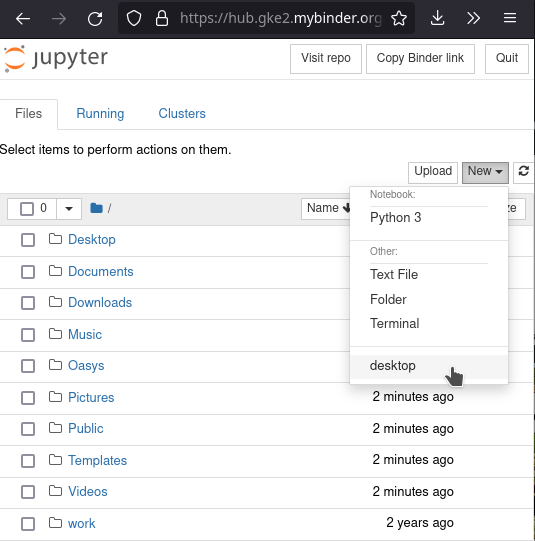
\includegraphics{figures/jupyter_select_desktop.png}
        \caption{}
        \label{fig:jupyter_select}
    \end{subfigure}
    \hfil
    \begin{subfigure}{0.5\textwidth}
        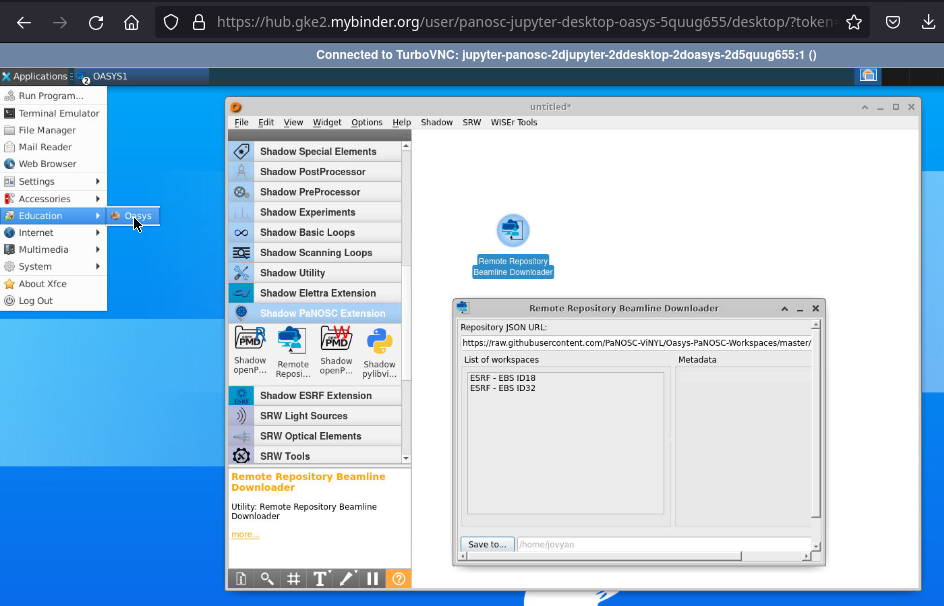
\includegraphics{figures/jupyter_oasys_run.png}
        \caption{}
        \label{fig:oasys_run}
    \end{subfigure}% trailing space between `subfigure` environments  had to be removed
    \caption{(a) Running the XFCE desktop environment from within Jupyter hub. (b) A new browser tab opens with XFCE desktop, providing a way to run OASYS inside the web browser while sharing the computing resources with the Jupyter hub instance.}
    \label{fig:oasysJupyter}
\end{figure}

OASYS projects are internally saved into the so-called \emph{OASYS Workspaces} (OWS). OWS files have an XML-like structure with the layout and some general properties being saved in easy-to-access ASCII format, while the actual content/parameters of individual widgets (optical elements) are in binary format (pickled Numpy objects). A beamline/instrument database therefore consists of a set of previously prepared and curated OWS files corresponding to an actual beamline. Each of the entries in the database contains some basic metadata and a pointer to the location of the respective OWS file. The user interacts with the database through a dedicated widget that is a part of the \emph{Shadow Panosc toolbox} extension.

The database itself consists of the actual OWS files and an index file and is hosted on Github. Since OWS files contain binary parts it is desirable not to change their content. Therefore an index file in JSON format is provided, serving two purposes:
\begin{itemize}
    \item user needs no Github account for read access,
    \item additional metadata can be provided.
\end{itemize}

The index file needs to be curated by the database admin and its changes can be easily tracked through the git commits. Furthermore, this way the widget offers the possibility of interacting with a database of arbitrary file formats and arbitrary locations, while still retaining the metadata. Figure \ref{fig:oasys_database} shows a screenshot of the widget. The links to the respective repositories are:

\begin{center}
\begin{tabular}{l l}
OASYS workspaces database & \url{https://github.com/PaNOSC-ViNYL/Oasys-PaNOSC-Workspaces} \\
OASYS Panosc toolbox code & \url{https://github.com/PaNOSC-ViNYL/OASYS1-PaNOSC}
\end{tabular}
\end{center}

\begin{figure}[htb]
    \centering
    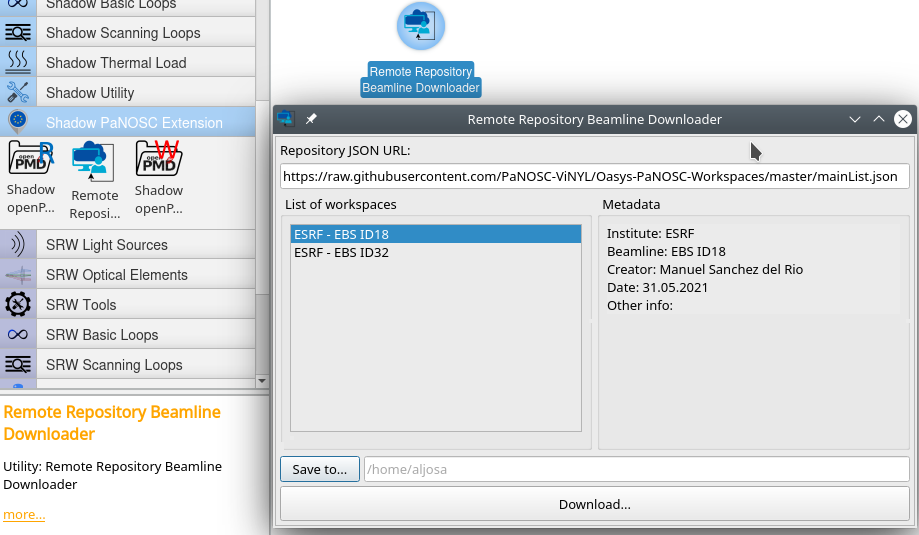
\includegraphics[width=0.52\textwidth]{figures/oasys_database_widget.png}
    \caption{OASYS widget for interaction with the online instrument database.}
    \label{fig:oasys_database}
\end{figure}

\section{McStasScript notebooks}
\label{sec:mcstas}
The McStasScript notebook repository along with the code repository are shown below, along with a link to the online documentation.
\begin{center}
\begin{tabular}{l l}
McStasScript code repo  & \url{https://github.com/PaNOSC-ViNYL/McStasScript} \\ 
McStasScript notebooks & \url{https://github.com/PaNOSC-ViNYL/McStasScript-notebooks} \\  
McStasScript documentation & \url{https://mads-bertelsen.github.io}
\end{tabular}
\end{center}
The McStasScript notebook repository currently contains a full 11 notebook
tutorial on McStas using the McStasScript Python interface developed under WP5.
This tutorial is also available through the online McStasScript documentation.
The repository also contains an example on using the widget interface for
McStasScript, and an example on using a cryostat construction tool included in
McStasScript.

\section{SimEx notebooks}
\label{sec:simex}
TBD: Jun, Carsten

As a part of the \emph{Shadow Panosc toolbox} an OASYS widget is being developed which allows for interoperability of SimEx and OASYS. The simulated X-ray wavefront output can be seamlessly connected to a SimEx calculator. Through the use of online Jupyter hub plugin for OASYS, the output can also be used in SimEx Jupyter notebooks. The middleware interface is built on saving the OASYS files into an openPMD-compliant hdf file (Panosc deliverable D5.1, task 5.1) and then read by the corresponding SimEx code. Figure \ref{fig:simex_oasys_widget} shows the widget within OASYS window.

\begin{figure}[htb]
    \centering
    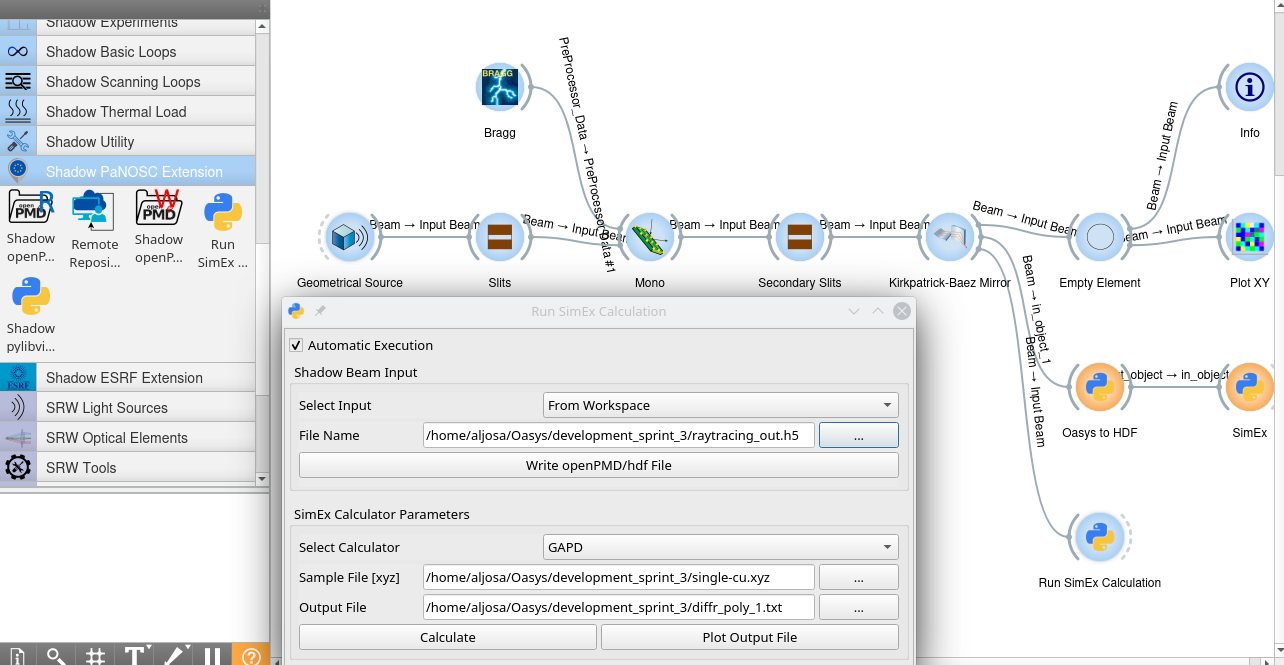
\includegraphics[width=0.75\textwidth]{figures/simexOasysWidget.png}
    \caption{OASYS widget which enables interoperability of OASYS output and SimEx calculators through an intermediate layer of using openPMD-compliant hdf files (developed previously).}
    \label{fig:simex_oasys_widget}
\end{figure}

\end{document}

